\section{Disk Arrangements}

\subsection{Oriented Realizations}
\subsection{Disk Packing Confinement Problem}
\begin{figure}[h]
\begin{center}
  ~ %add desired spacing between images, e. g. ~, \quad, \qquad etc.
    %(or a blank line to force the subfigure onto a new line)
  \begin{subfigure}[b]{0.1\textwidth}
	  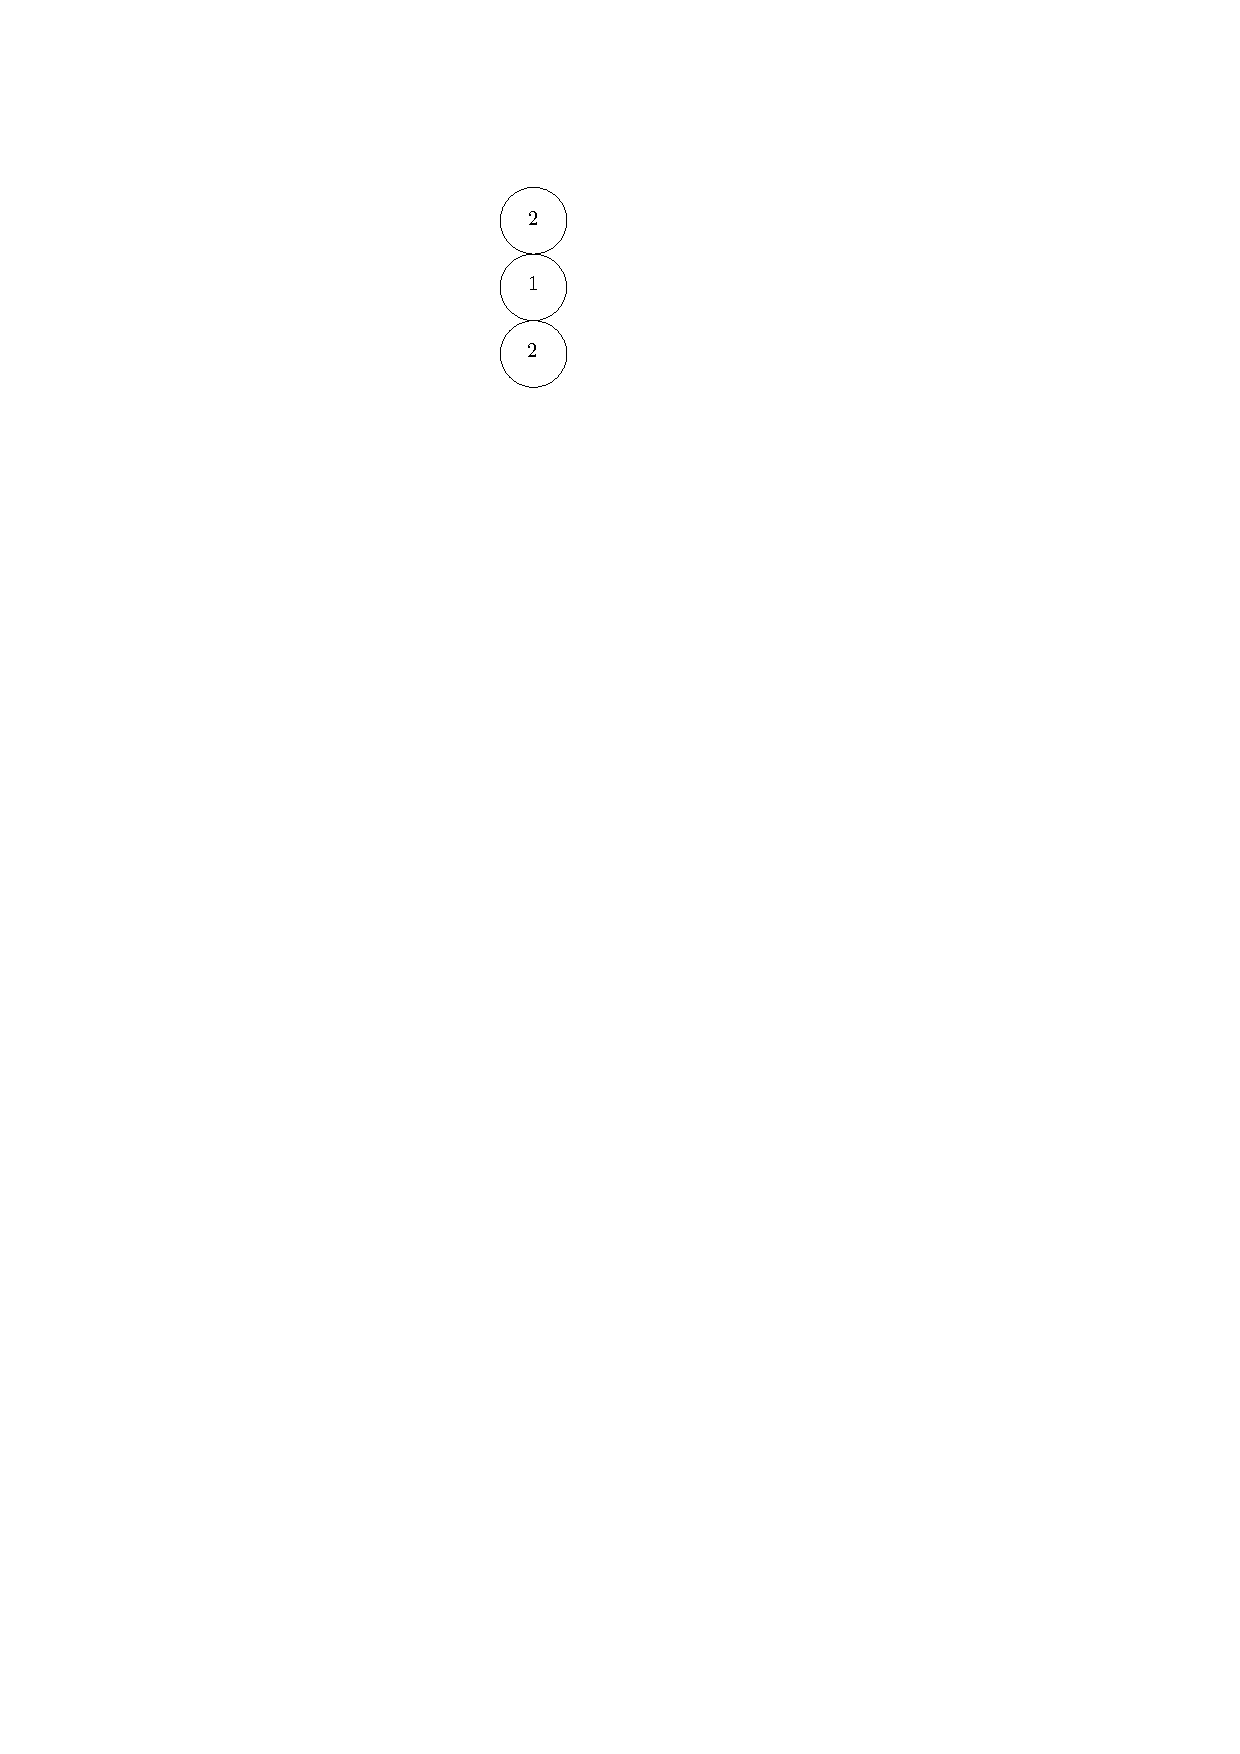
\includegraphics[width=\textwidth]{graphics/degree2arrangement.pdf}
	  \caption{A disk arrangement with two layers of disks}
	  \label{fig:linkage-1-1}
  \end{subfigure}
  \begin{subfigure}[b]{0.4\textwidth}
	  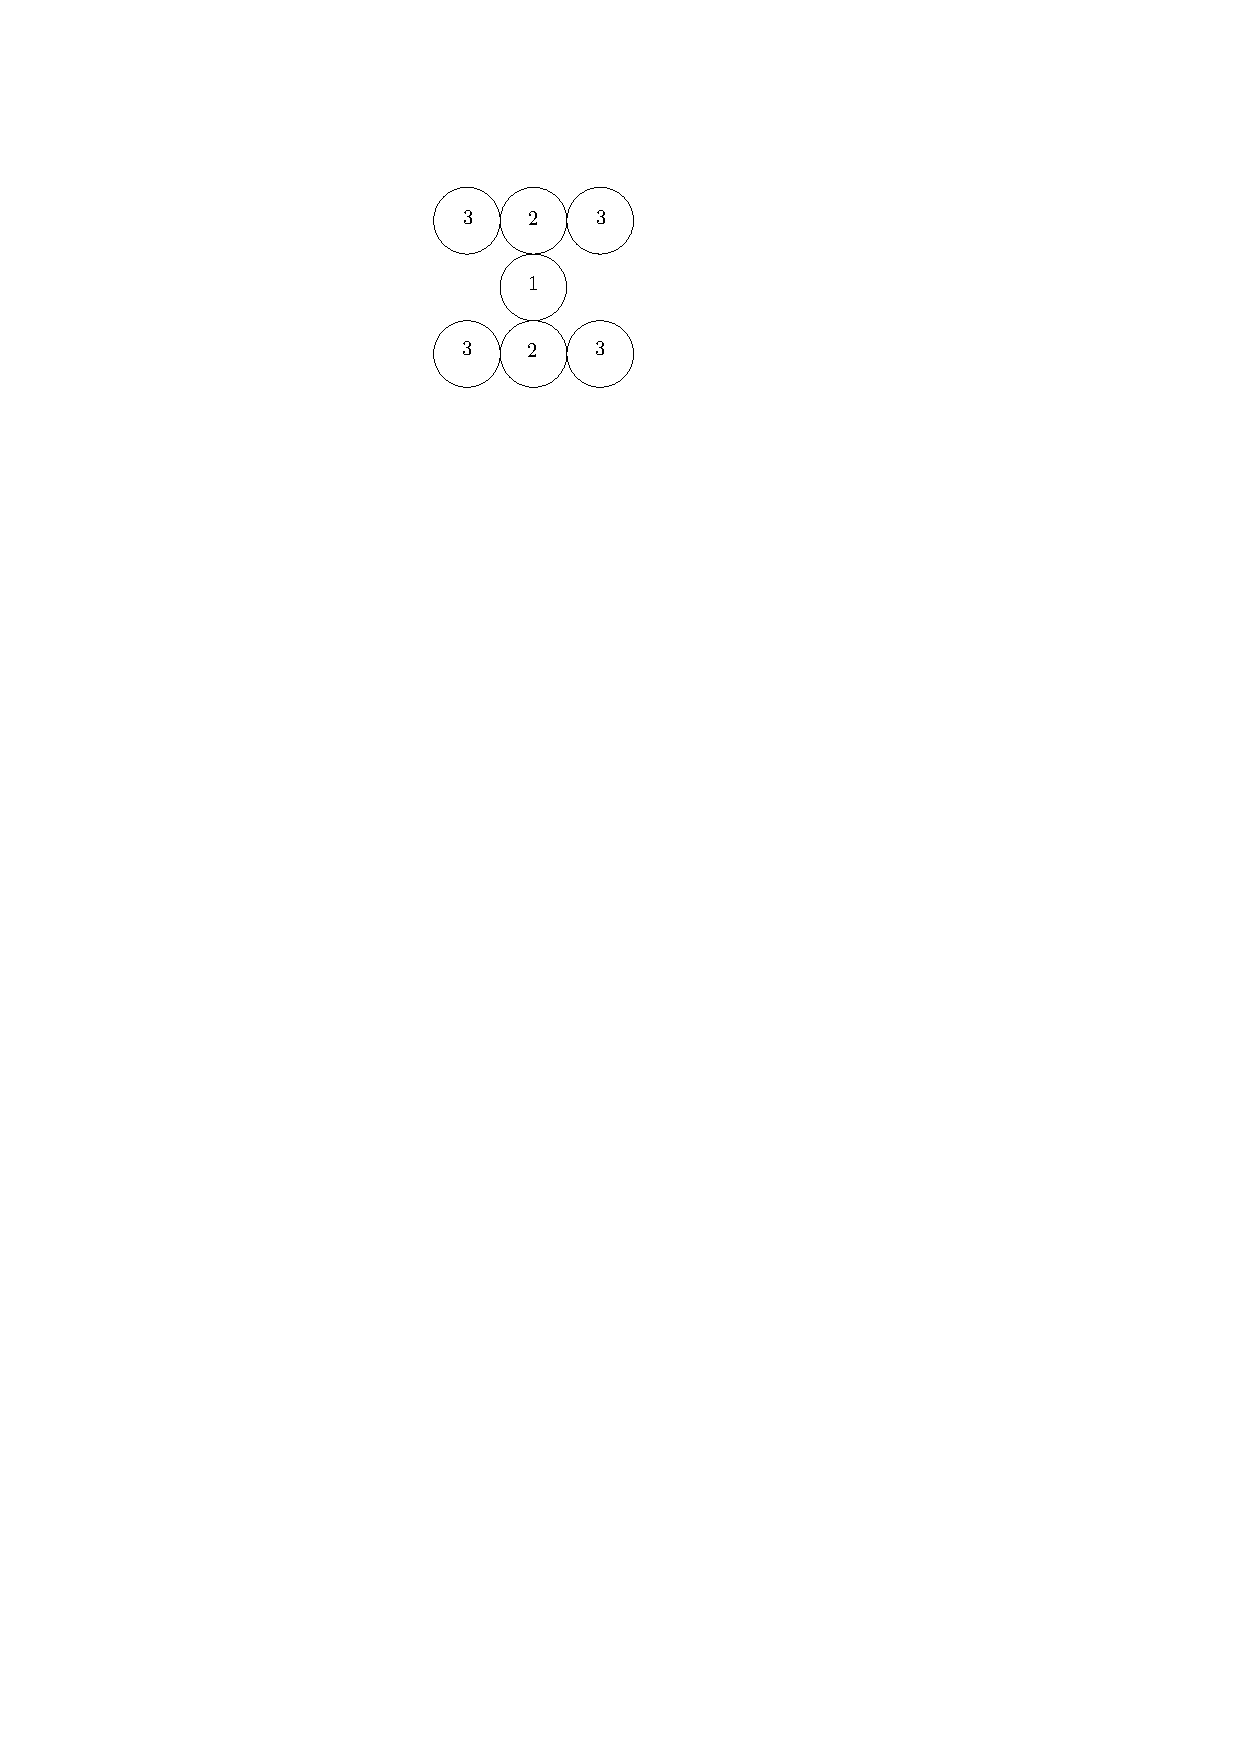
\includegraphics[width=\textwidth]{graphics/degree3arrangement.pdf}
	  \caption{A disk arrangement with three layers of disks}
	  \label{fig:circlePacking1-2}
  \end{subfigure}
  \begin{subfigure}[b]{0.4\textwidth}
	  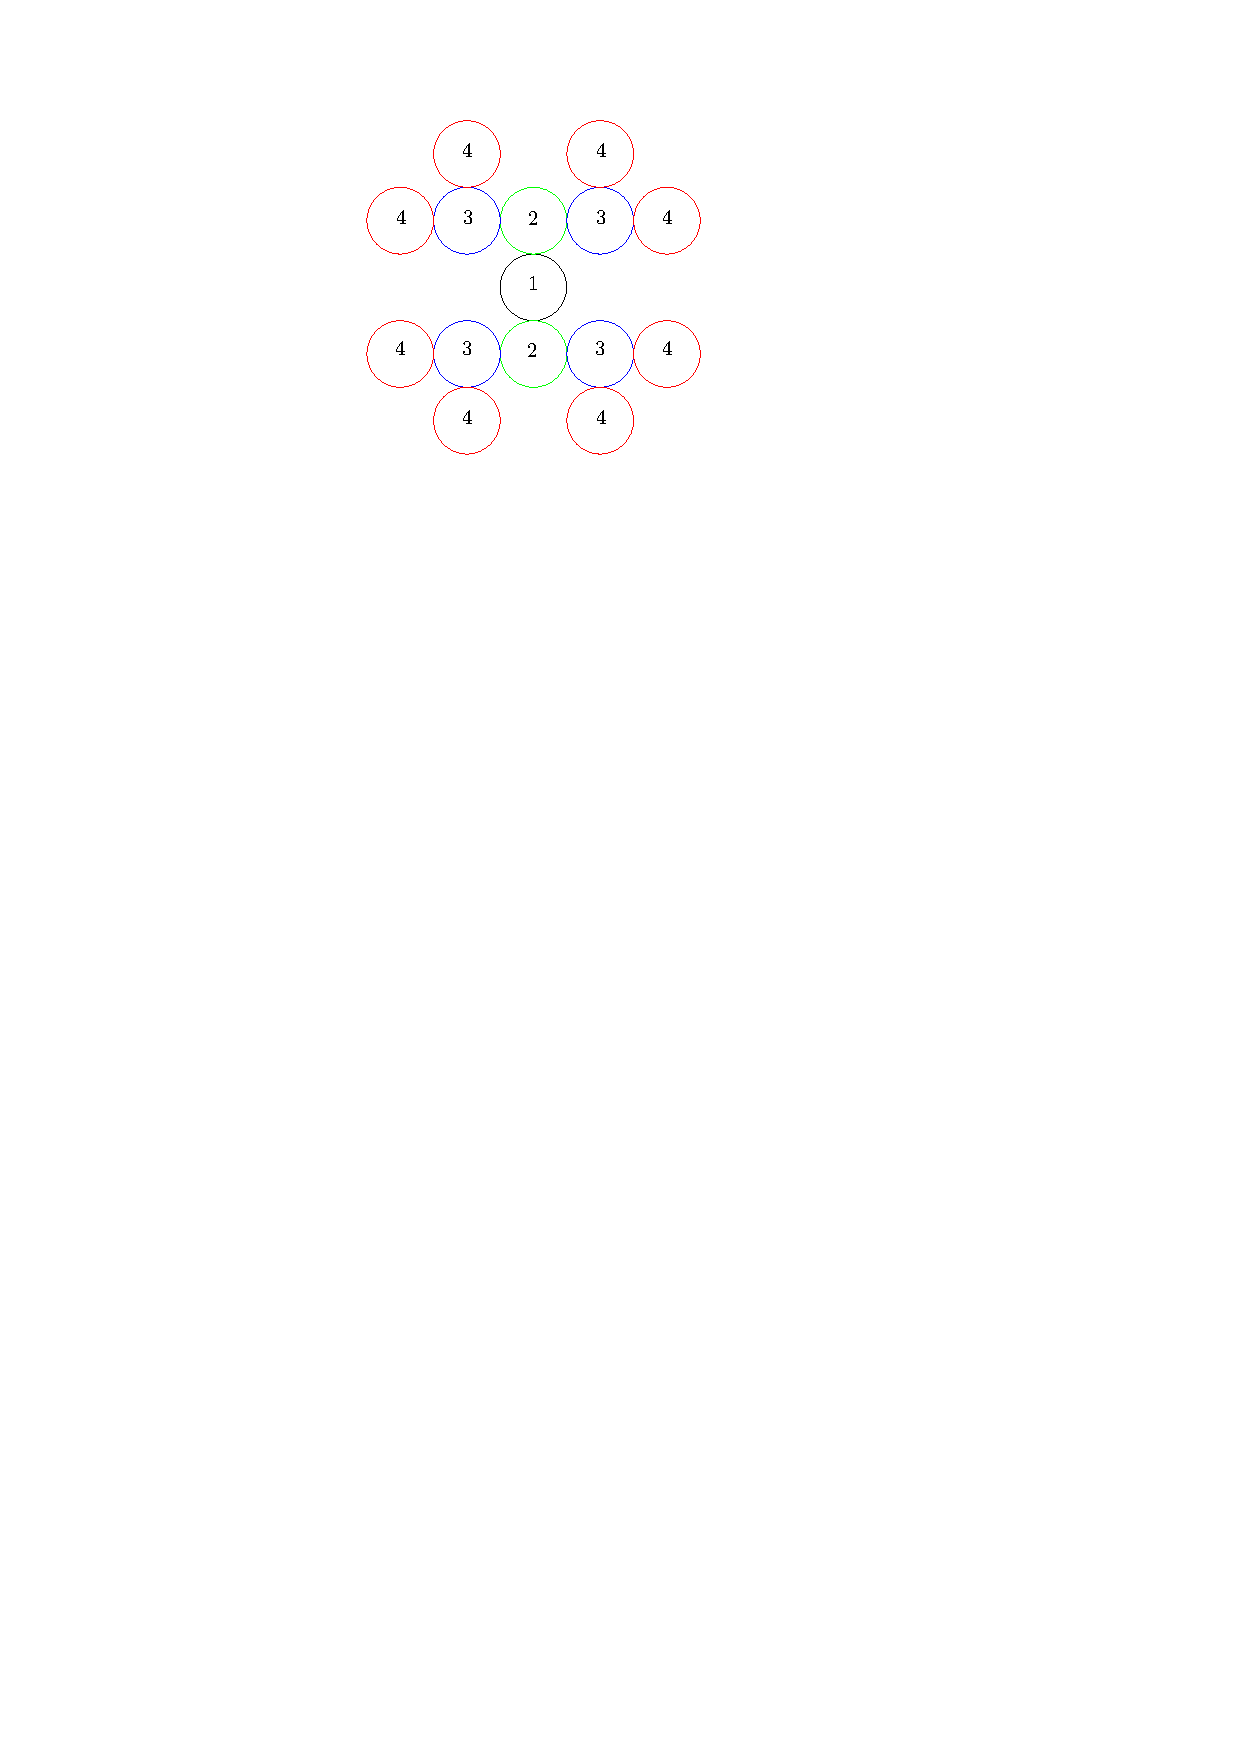
\includegraphics[width=\textwidth]{graphics/degree4arrangement.pdf}
	  \caption{A disk arrangement with four layers of disks}
	  \label{fig:circlePacking1-2}
  \end{subfigure}
\end{center} 
\caption{The gradual growth of disk arrangements by adding two kissing disks to each of the previously generated disks.  By continuing this arrangement growth, the space needed to contain the kissing disks will exceed the area containing the disk arrangements.}\label{fig:circlePacking-1}
\end{figure}
